% Chapter 6

\chapter{Data processing and display of obtained parameters of MOS structures.}\label{Chapter6}
\lhead{Chapter 6. \emph{Data Processing and display of MOS structures parameters}}

In this chapter we briefly describe the procedure for processing the
data measured using data acquisition programs and we will focus on the
plan view of the obtained parameters of the MOS
structures. Methodology of parameter calculation of the MOS structures
has been described in Chapters 3 and 4, to which we will will be
referred to.

Most of the parameters are determined from the measured data using
separate programs and stored in data files whose structure has been
described in Section 5. Area distribution of the calculated parameter
structures MOS can then be displayed on a computer display. When
displayed on display, 16 colors are available, but when displaying
the images on the printer, only 6 colors. The orientation of the
silicon wafer in the images is towards the `facet up', with one square
of the displayed area representing the value of of the MOS structure
parameter. The color of the square depends on the interval to which
the value falls. The range of intervals is shown in the right part of
the figure, with the number given for each color represents the lower
limit of the interval. Because the colors in the scale of the
intervals are repeated several times, it was necessary to indicate in
which intervals in which the displayed values are located. This is
indicated by a capital letter `X' between the lower boundary of the
interval and the adjacent color. It may still be noted that randomly
different results in some points on the silicon slab will cause them
to be different in the range of intervals a marked interval will
appear which is apparently unrelated to the other values, which can be
attributed to the non-functional structure of MOS\@. It is still
necessary to note that the orientation of the scale may change when
displaying different parameters may vary.

\section{Determination of the concentration profile of the dopant impurities, implantation dose and tension of the aligned strips.}\label{sec:6.1}

Determination of the concentration profile of the interfering
admixtures is performed by a separate program which requires as input
data sets of (a) measured HF C-V dependencies and (b) the measured
capacitances of the oxide layer of the structure MOS\@. The output of
the program is a data file containing the depth curves
concentration profiles of the investigated MOS structures, which are
calculated according to the relations given in
Section~\ref{sec:4.1}. If, in the process of collection data
collection process, the program performs a correction for the
quasi-static C-V dependence the concentration profile to the interface
trap density $Si-SiO_2$. The surface potential is determined according
to the equations~\ref{eq:4.3} and~\ref{eq:4.4} and use it to correct
the deep depletion at the semiconductor surface and for calculating
the depth (width SCR). The by-product is a dataset containing the
voltages of the aligned $V_{fb}$ bands, which are determined at the
C-V dependence point, for for which the surface potential $\varphi_s$
varies sign. Figure~\ref{fig:6.1} represents the surface distribution
of concentration at different depths in the semiconductor, and
Figure~\ref{fig:6.2} shows the distribution of $V_{fb}$. The
concentration profile of the impurities was created by implanting
$P^{31}$ with a dose of $4.0 \times 10^{15} m^{-2}$ at an energy of
$120 keV$. The activation was carried out for 40 minutes at
temperature $1050 \degree C$ in a $N_2$ atmosphere. The mean value of
$N(x)$ together with other curves for different implant doses are
shown in Figure~\ref{fig:7.3}.

For the known concentration profile curves, we can calculate the
dose of implantation according to the relationship

\begin{equation}\label{eq:6.1}
  D = \int_{0}^{x_{1}}(N(x) - N_{b}) dx
\end{equation}

,where we assume that we know the progression of $N(x)$ up to distance
$x_{1}$, for which

\begin{equation}\label{eq:6.2}
  N(x) = N_{b} \qquad {x \ge x_{1}}
\end{equation}

The dose $D$ calculated in this way represents the fraction of
implanted of ions that entered the semiconductor during implantation
and were activated in the post-implantation heat treatment. At
Figure~\ref{fig:6.3} shows the areal distribution of the dose to
silicon wafer tested, determined from the $N(x)$ dependence shown in
Figure~\ref{fig:6.1}.

\begin{figure}[h!]\centering
  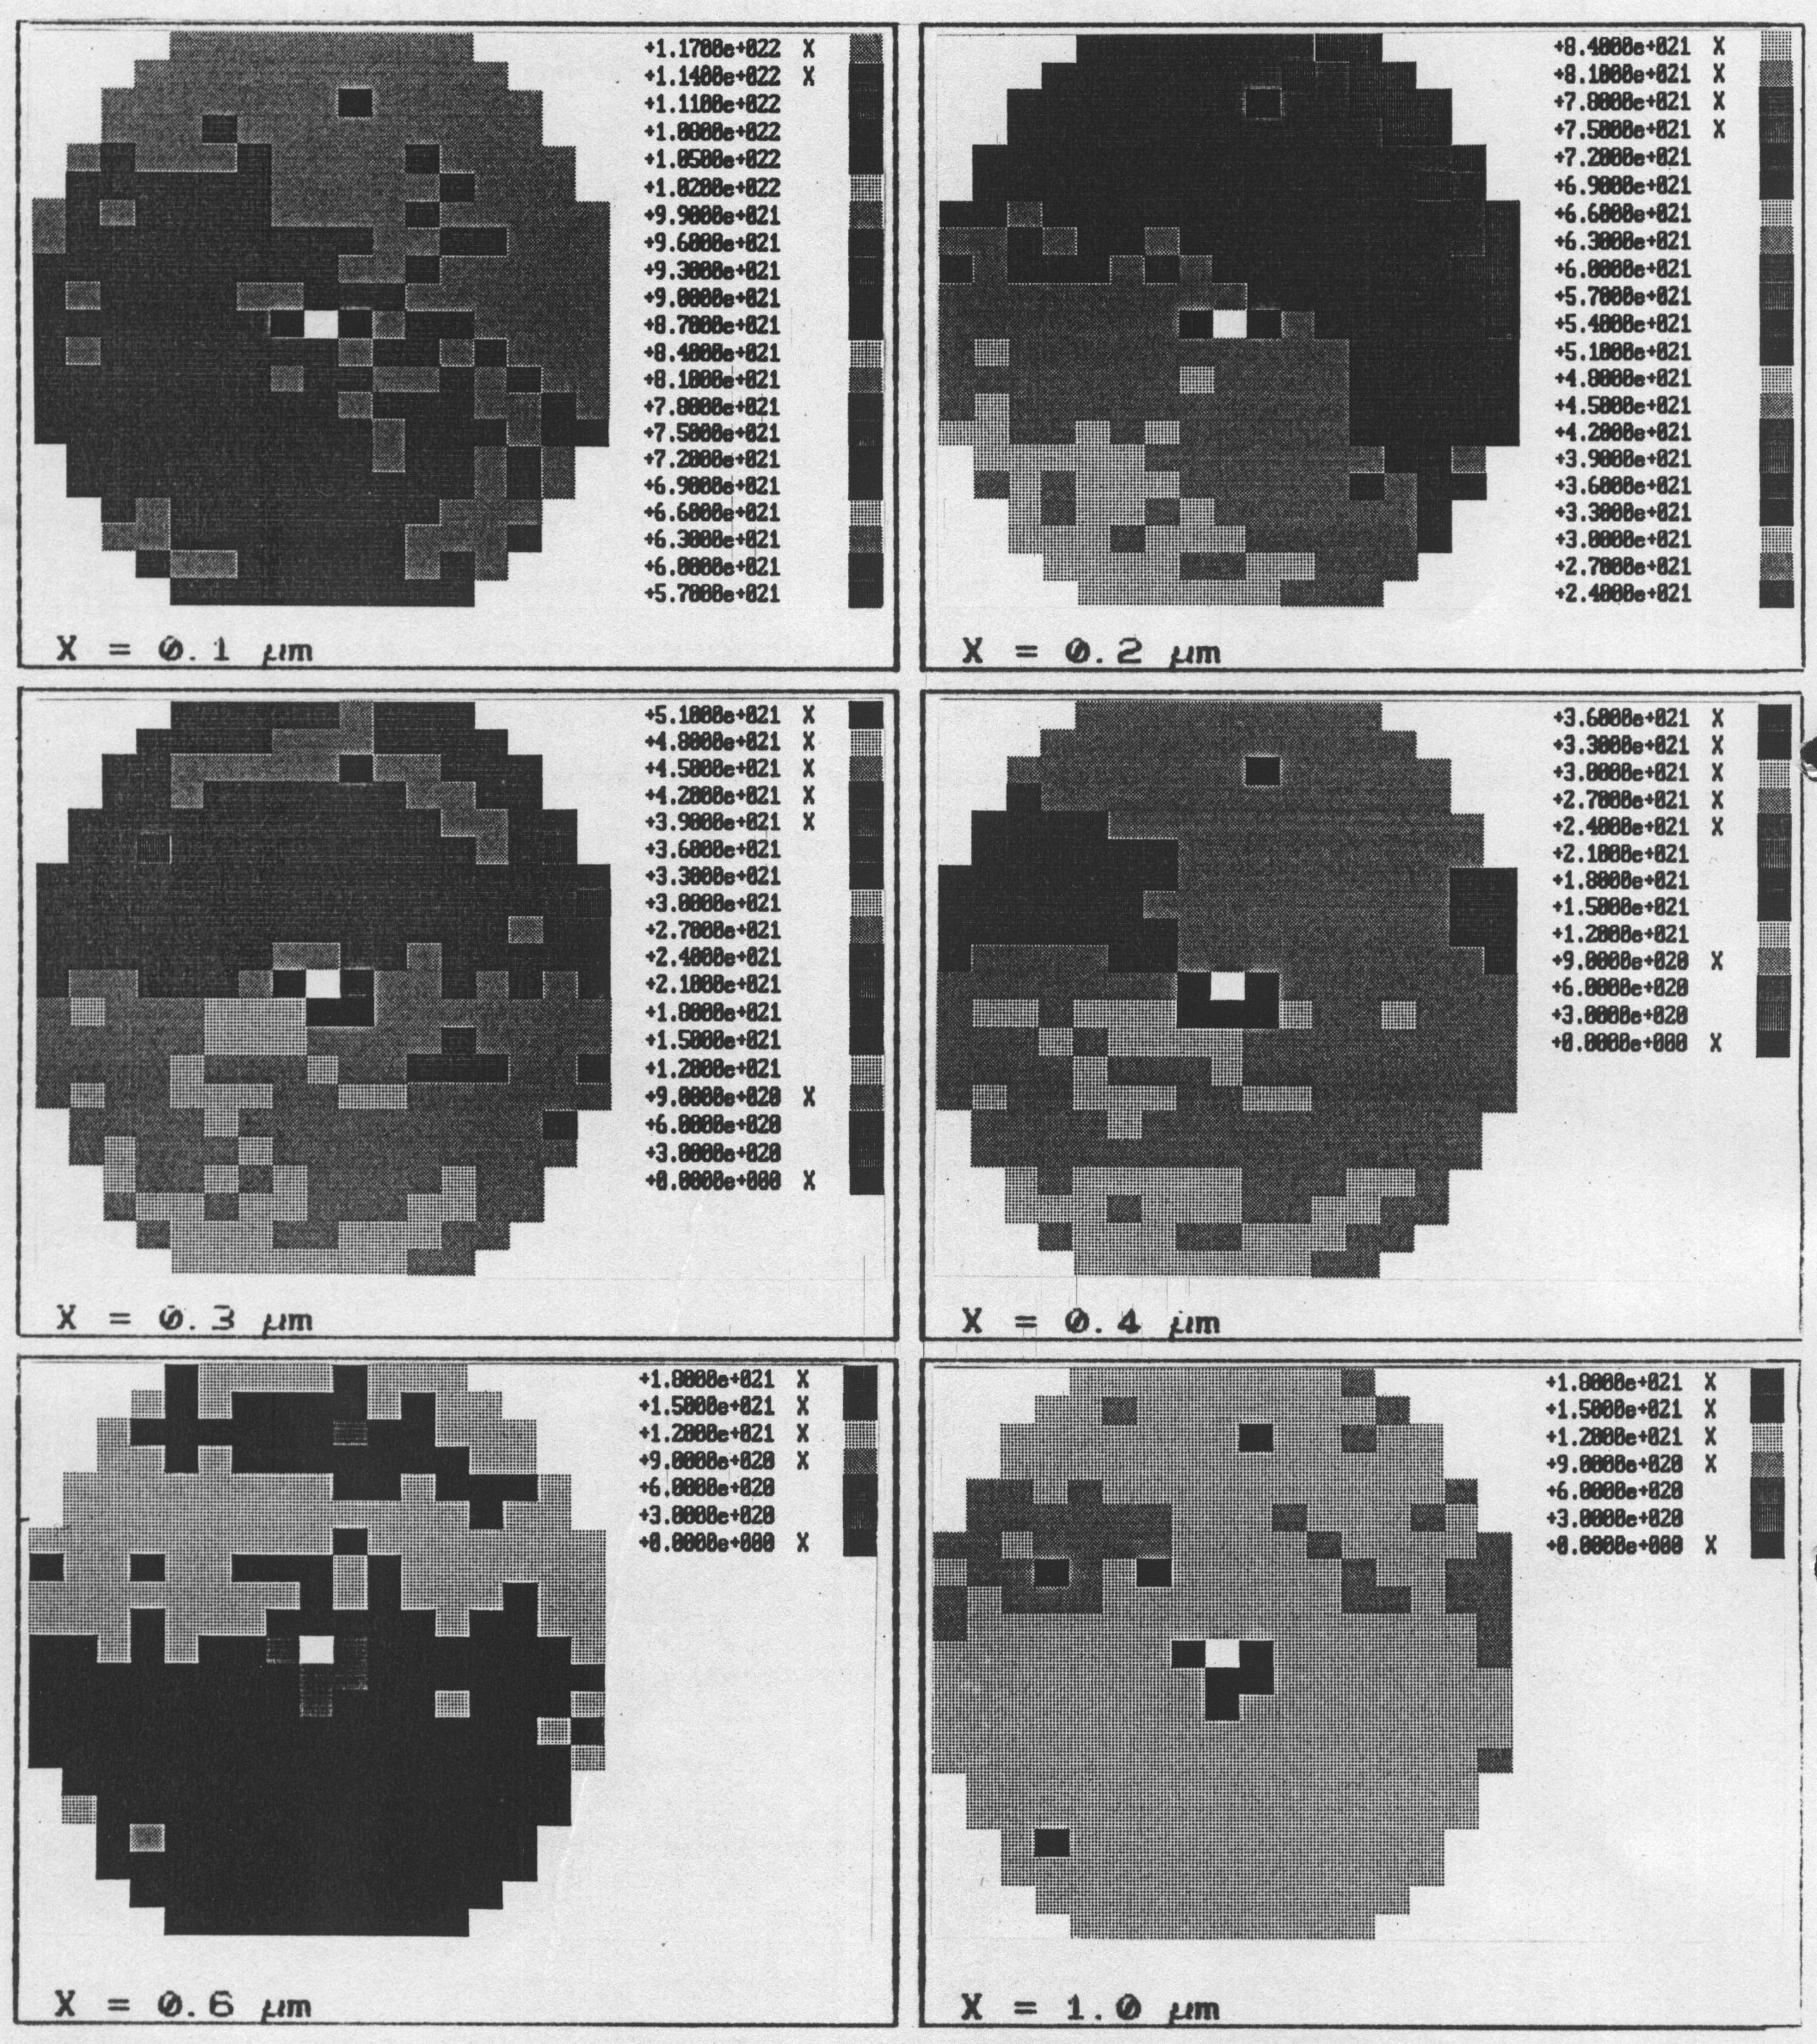
\includegraphics{Figures/fig-6-1.eps}% chktex-file 8
  \caption[The distribution of tangents $N(x)$ at different depths
    $x$]{Distribution of the intervening admixtures $N(x)$ at
    different depths $x$ below the semiconductor surface for an
    implantation dose of $4.0 \times 10^{15}m^{-2}$.}\label{fig:6.1}
\end{figure}

\begin{figure}[h!]\centering
  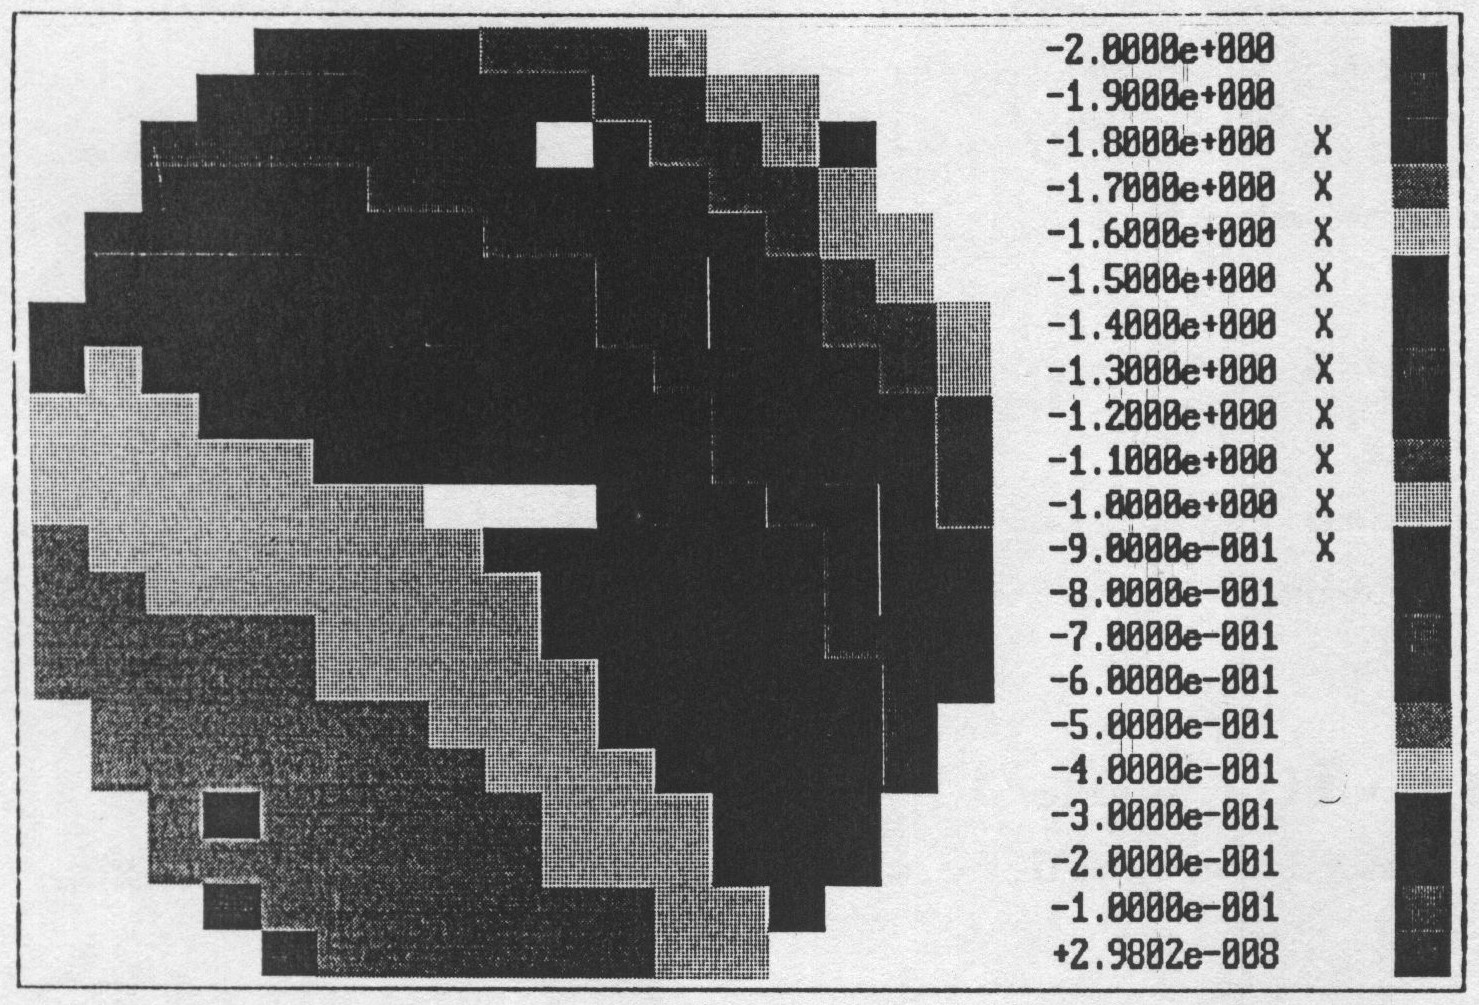
\includegraphics{Figures/fig-6-2.eps}
  \caption[Surface layout $V_{fb}$]{Surface layout $V_{fb}$ determined
    by calculating $N(x)$ from Figure~\ref{fig:6.1}.}\label{fig:6.2}
\end{figure}

\begin{figure}[h!]\centering
  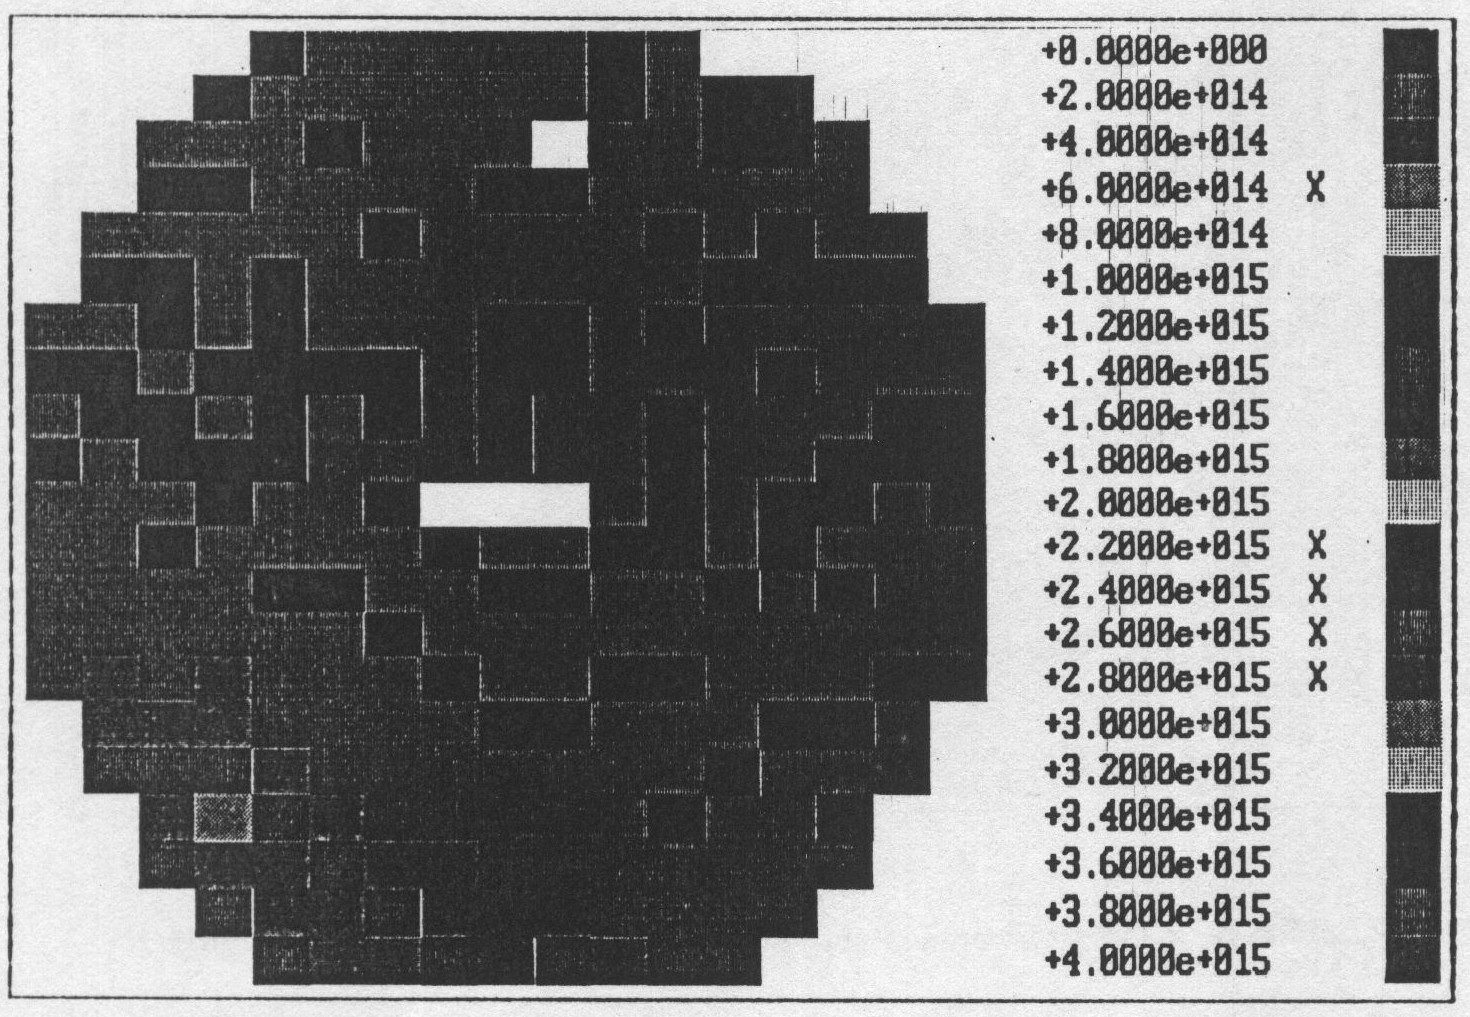
\includegraphics{Figures/fig-6-3.eps}
  \caption[Area distribution of measured implantation dose]{Area
    distribution of measured implantation dose for profile $N(x)$
    Figure~\ref{fig:6.1}.}\label{fig:6.3}
\end{figure}

\section{Oxide layer thickness determination.}\label{sec:6.2}

If we know the capacity of the oxide layer of the MOS structure and
its area, then we can calculate its thickness according to the
relation

\begin{equation}\label{eq:6.3}
  h_{ox} = A \frac{\epsilon}{C_{ox}}
\end{equation}

where we used the relative permittivity value $SiO_{2}$
$\epsilon_{r}=3.9$. The area distribution of the oxide layer thickness
is then is shown in figure~\ref{fig:6.4}.

\begin{figure}[h!]\centering
  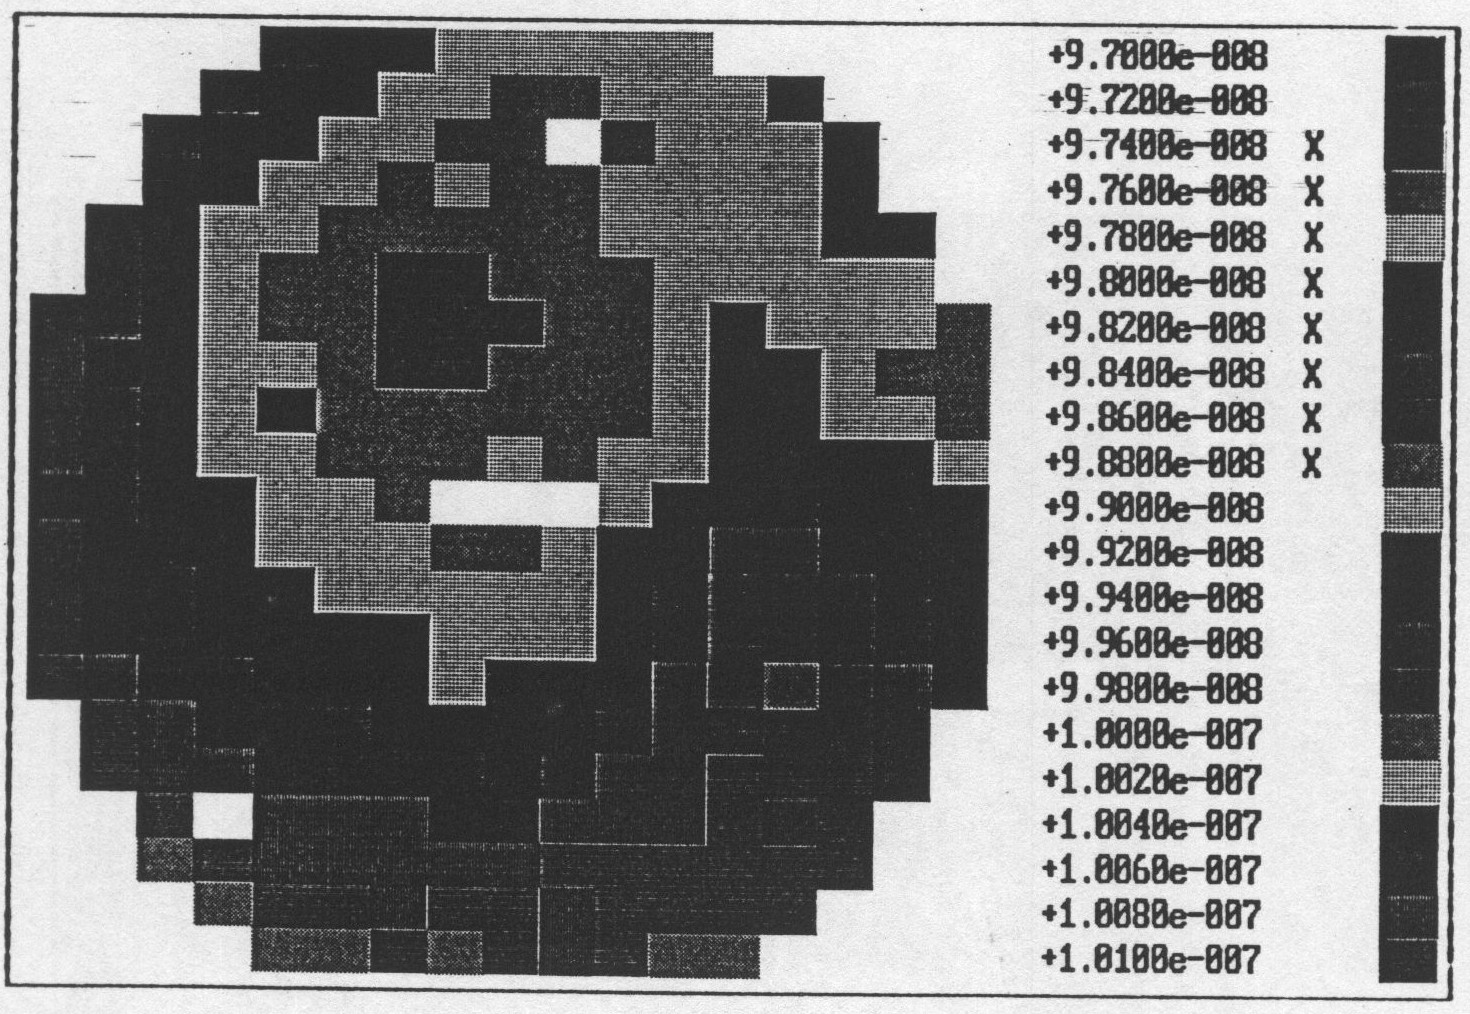
\includegraphics{Figures/fig-6-4.eps}
  \caption[Plane distribution of the thickness of the $h_{ox}$]{Figure
    distribution of the thickness of $h_{ox}$.}\label{fig:6.4}
\end{figure}

\section{Density determination of $Si-SiO_{2}$ interface traps.}\label{sec:6.3}

To calculate the interface trap density, we use the comparison of HF and
quasi-static C-V dependence, using the procedure described in
Section~\ref{sec:4.2.1}. It may be noted that to determine the position of the Fermi
level on the semiconductor surface, we use the values of the surface potential
$\varphi_{s}(V_{g})$, obtained by integrating the quasi-static C-V
dependence and the value of the integration constant $\varphi_{s0}$ is determined
by the procedure described in Appendix~\ref{app:AppendixG}.

The whole procedure of calculating $D_{it}$ is implemented by two
programs. The first program, based on the measured quasi-static C-V
dependencies and the known $N(x)$ depth curves, it computes the
dependencies $\varphi_{s}(V_{g})$, which it stores in a data file. The
second program requires data files

\begin{itemize}
\item HF C-V dependencies $C_{mos}^{HF}(V_{g})$
\item quasi-static C-V dependence $C_{mos}^{LF}(V_{g})$
\item dependence of the surface potential on the gate voltage $\varphi_{s}(V_{g})$.
\end{itemize}

Calculated values of $D_{it}$ as a dependence of the Fermi surface
position in in the forbidden band of the semiconductor shall be stored
in the data file. At Figure~\ref{fig:6.5} shows the area distribution
of $D_{it}$ in the center of the forbidden band.

\begin{figure}[h!]\centering
  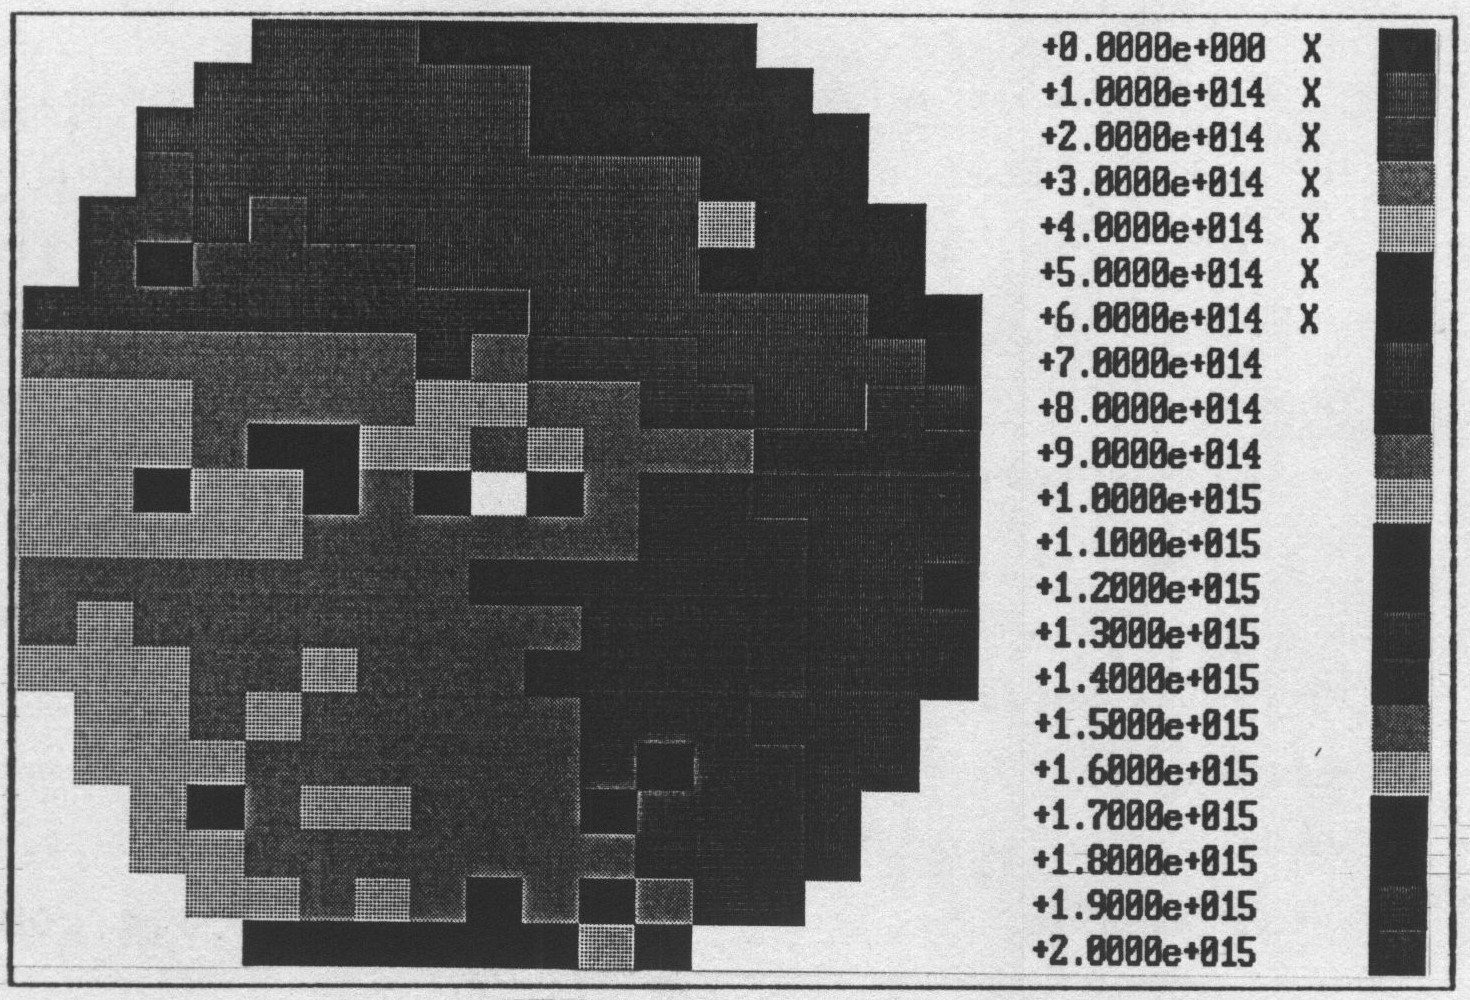
\includegraphics{Figures/fig-6-5.eps}
  \caption[Area density distribution of $Si-SiO_{2}$ interface traps
    in center of the forbidden band]{Area density distribution of
    interface traps $Si-SiO_{2}$ in the center of the forbidden
    band.}\label{fig:6.5}
\end{figure}

\section{Generational lifetime of minority charge carriers.}\label{sec:6.4}

In the process of data collection by the constant-width SCR method, a
data file containing $V_{g}(t)$ dependency directives for different
SCR widths for the tested MOS silicon wafer structures. To determine
the generation lifetime of the minority charge carriers according to
the equation~\ref{eq:3.10} is important is how we calculate the
derivative of the dependence of the $V_{g}(t)$ directions by the
distance of the SCR boundary from the semiconductor surface. Using
numerical filters is not appropriate in this case because we have few
dependence points $dV_{g}/dt = f(w)$. In this case we can use
approximation by local polynomials. Theoretical basis and source text
of the procedure in Algol is given, for example, in~\cite{6.1}. At
Figure~\ref{fig:6.6} shows the area distribution of the generation
time of minority charge carriers, representing its mean value in the
region from $0.9\mu m$ to $1.3\mu m$.

\begin{figure}[h!]\centering
  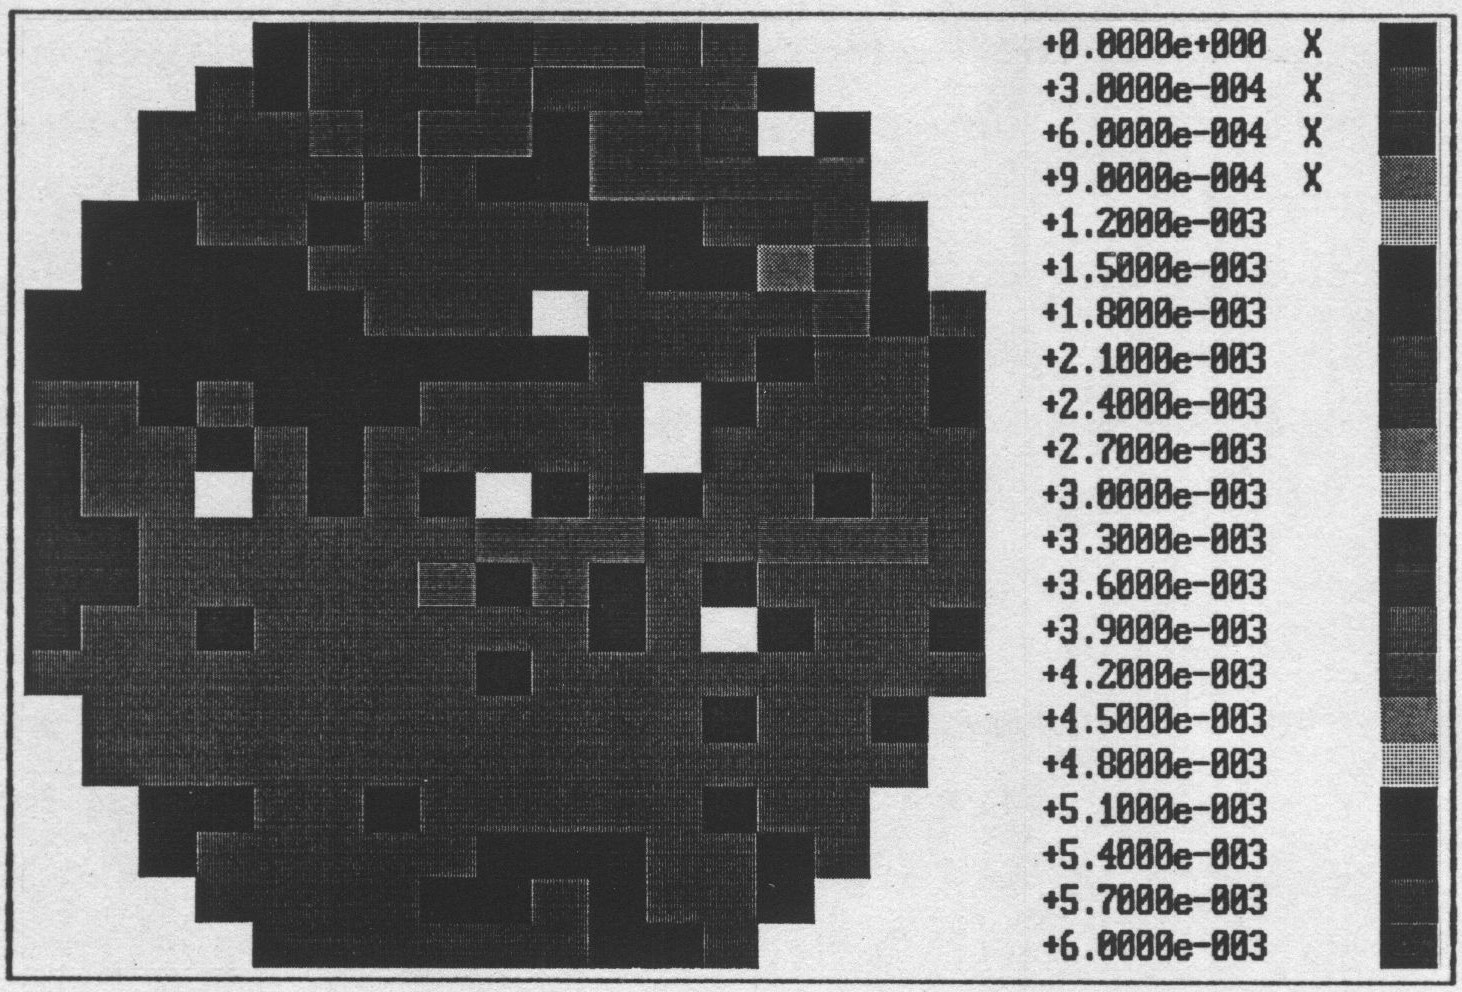
\includegraphics{Figures/fig-6-6.eps}
  \caption[Area distribution of the generational lifetime of minority
    charge carriers]{Area distribution of the generational lifetime of
    minority charge carriers for the semiconductor region from $0.9
    \mu m$ to $1.3 \mu m$.}\label{fig:6.6}
\end{figure}

\begin{thebibliography}{}
\bibitem{6.1}{6.1}
  Ludwig R.: Methoden der Fehler und Ausgleichrechnung. VEB Berlin 1969.\ p.103.
\end{thebibliography}
